\documentclass[aspectratio=169,xcolor=table]{beamer}

% --- Pacchetti ---
\usepackage[utf8]{inputenc}
\usepackage[T1]{fontenc}
\usepackage[italian]{babel}
\usepackage{lmodern}
\usepackage{graphicx}
\usepackage{booktabs}
\usepackage{xcolor}
\usepackage{amsmath, amssymb}

% --- Configurazione Tema (Madrid elegante con colore personalizzato) ---
\usetheme{Madrid}
\definecolor{unimeblue}{RGB}{12, 35, 64} % Blu scuro istituzionale
\usecolortheme[named=unimeblue]{structure}

% --- Informazioni ---
\title[Lab IA - Progetto 1]{Progetto 1: Segmentazione Clienti e Churn Prediction}
\subtitle{Spiegazione Semplificata del Progetto}
\author[Massimo Mantineo]{Massimo Mantineo\\{\small Matricola: 541924}}
\institute[Unime MIFT]{
  Università degli Studi di Messina\\
  Corso di Laurea in Informatica
}
\date[A.A. 2025/2026]{Laboratorio di Intelligenza Artificiale\\A.A. 2025/2026}

% Logo nel titolo
\titlegraphic{
\includegraphics[width=3cm]{logo_unime_orizontale.png}}

\begin{document}

% Slide 1: Titolo
\begin{frame}
  \titlepage
\end{frame}

% Slide 2: Obiettivi e Dataset
\begin{frame}{1. Di cosa tratta il Progetto e da dove vengono i Dati?}
  \begin{columns}
    \begin{column}{0.55\textwidth}
      \textbf{Il Dataset:}
      \begin{itemize}
        \item Usiamo il dataset reale \textbf{Telco Customer Churn di IBM}.
        \item Contiene i profili commerciali e anagrafici di 7043 clienti.
      \end{itemize}
      \vspace{0.2cm}
      \textbf{L'obiettivo:}
      \begin{itemize}
        \item Capire quali clienti rischiano di abbandonare l'operatore (\textbf{Churn Prediction}) per intervenire in tempo.
      \end{itemize}
      \vspace{0.2cm}
      \textbf{La sproporzione delle classi:}
      \begin{itemize}
        \item Le classi sono sbilanciate (3:1): 73.4\% fedeli e 26.6\% che abbandonano.
      \end{itemize}
    \end{column}
    \begin{column}{0.43\textwidth}
      \centering
      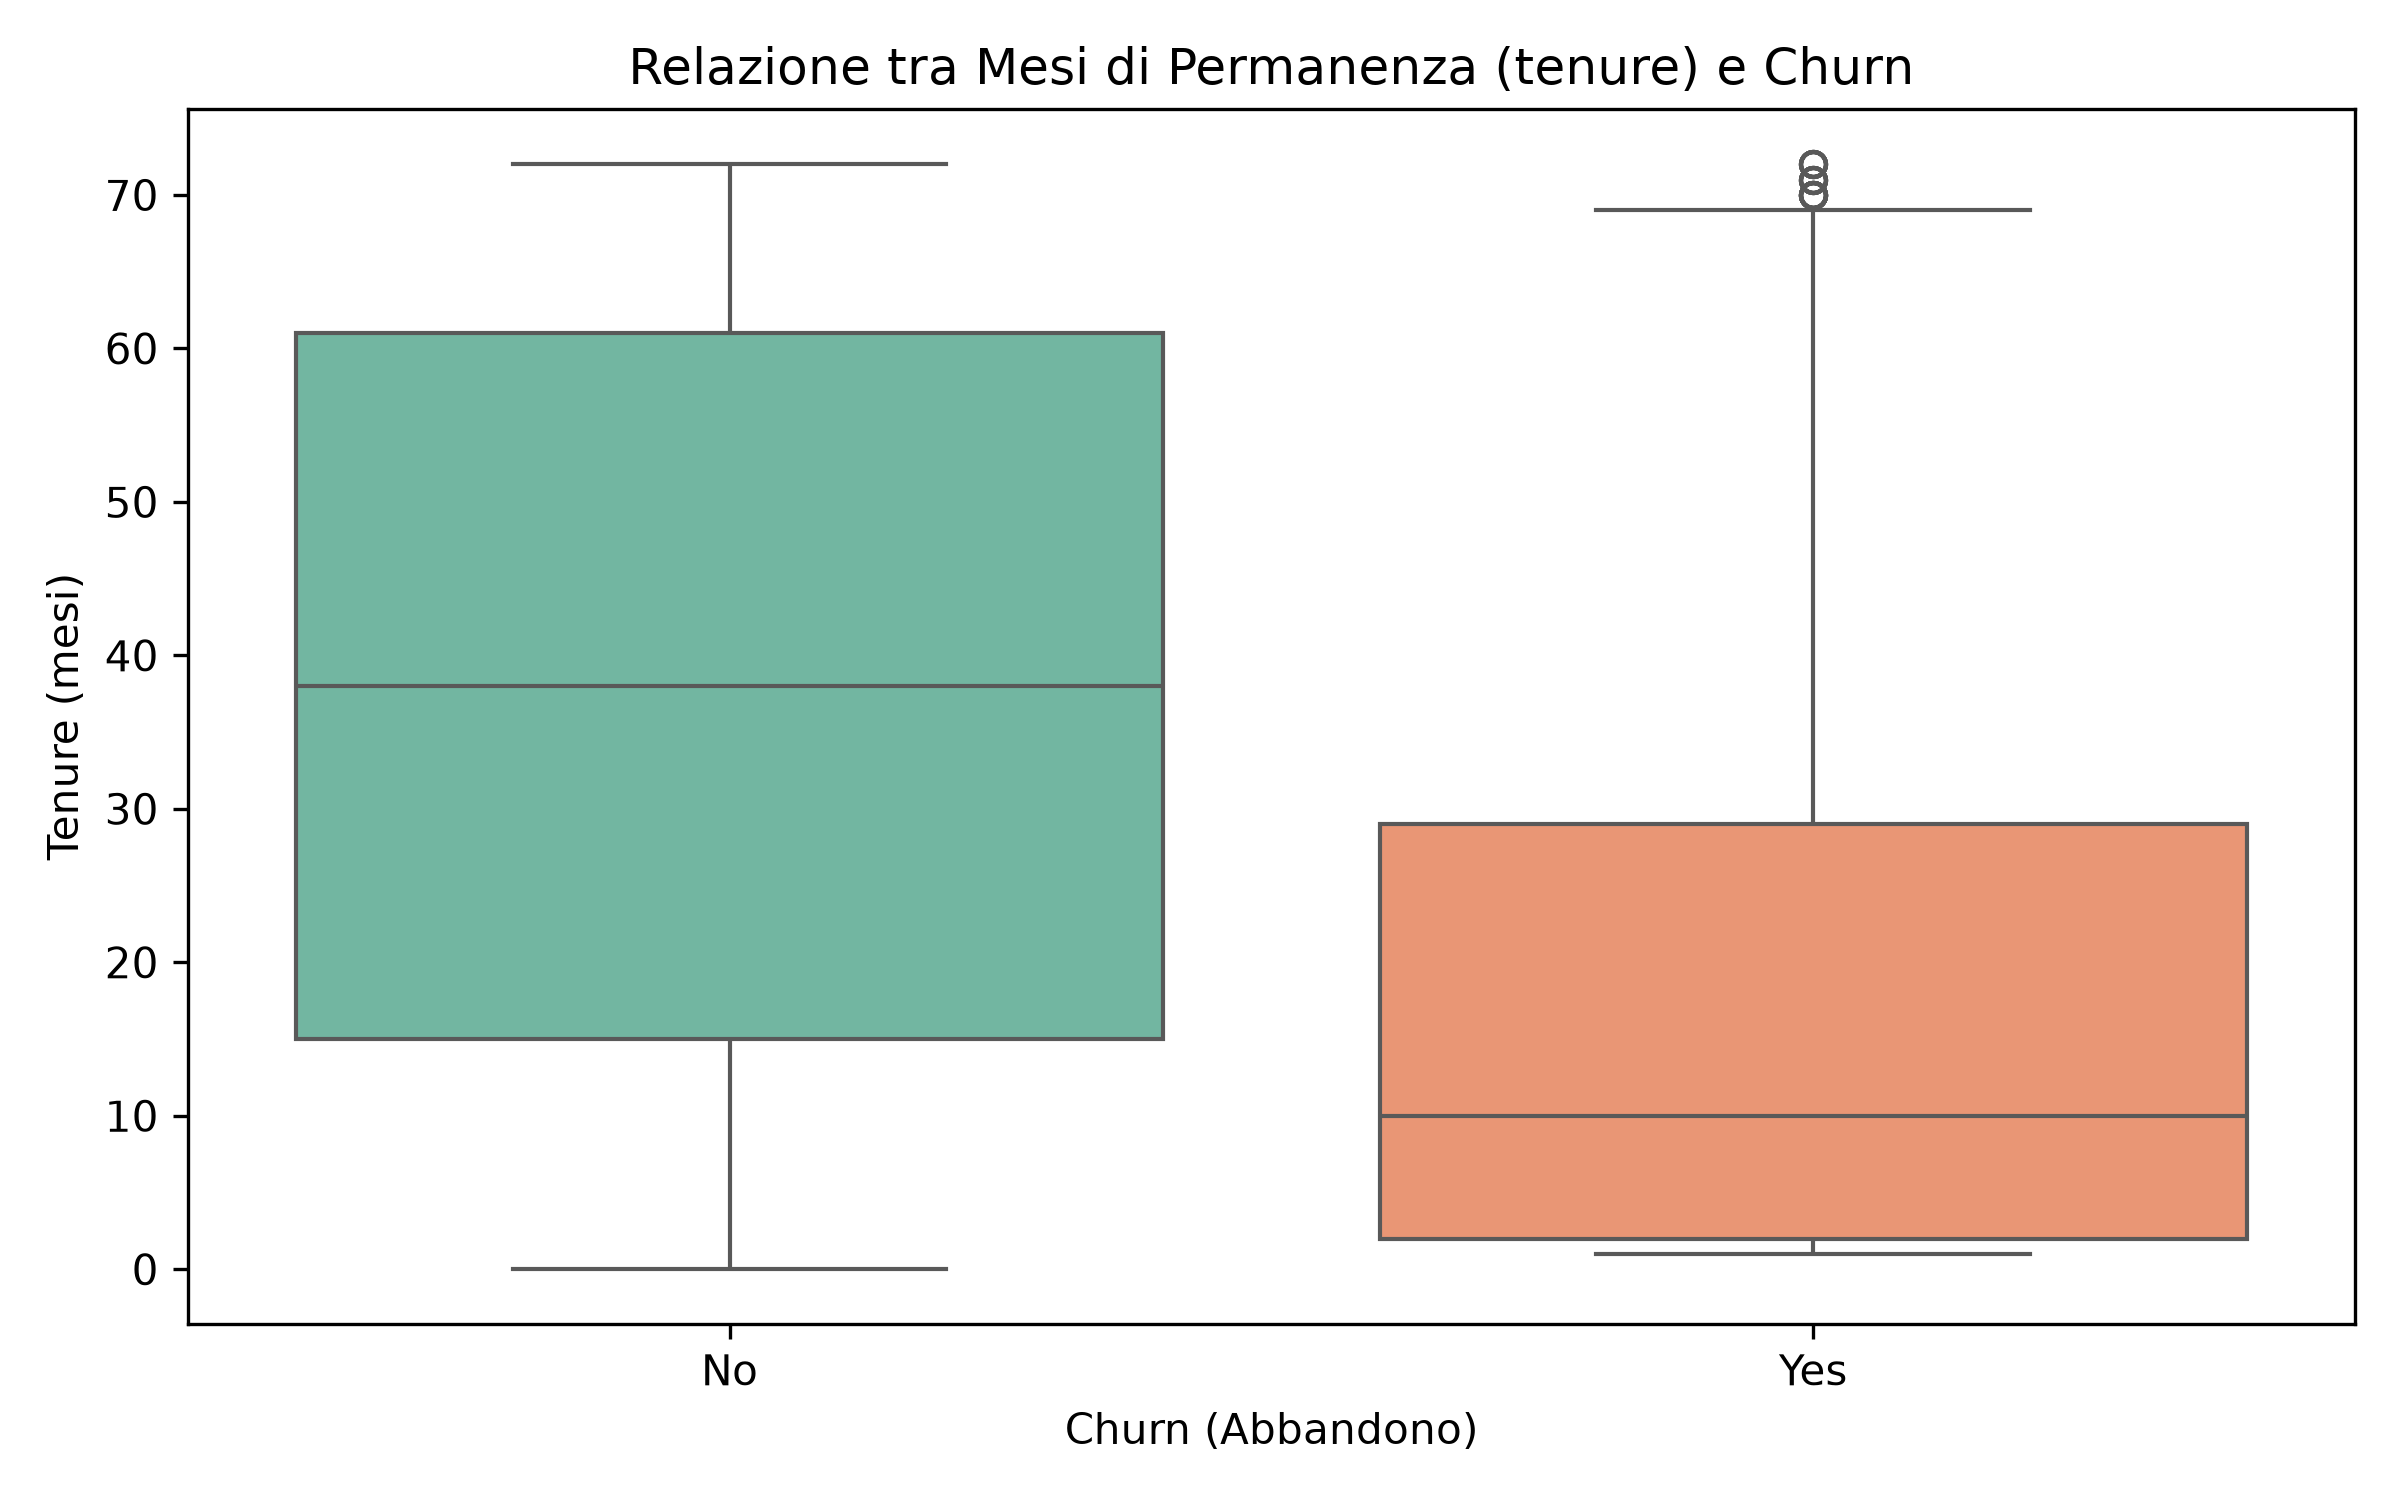
\includegraphics[width=0.9\textwidth]{../grafici/churn_vs_tenure.png}
      \begin{center}\scriptsize \textbf{Grafico}: Chi se ne va (Yes Churn) ha una permanenza bassissima (mediana $\approx$ 10 mesi).\end{center}
    \end{column}
  \end{columns}
\end{frame}

% Slide 3: Preprocessing dei Dati
\begin{frame}{2. Come abbiamo sistemato i Dati? (Preprocessing)}
  \small
  Per preparare i dati ai modelli ho seguito cinque passi fondamentali:
  \vspace{0.2cm}
  \begin{itemize}
    \item \textbf{Celle vuote}: Riempite 11 celle vuote in \textit{TotalCharges} con \texttt{0.0} (erano nuovi clienti con tenure=0 che non avevano ancora ricevuto bollette) e convertito in float.
    \item \textbf{Rimozione customerID}: ID rimosso perché non ha valore predittivo ed eviterà l'overfitting su codici casuali.
    \item \textbf{One-Hot Encoding}: Tradotto le parole in numeri (0/1). Usato \texttt{drop\_first=True} (escludendo una categoria) per evitare ridondanze matematiche (multicollinearità).
    \item \textbf{Standard Scaling}: Riportato le variabili numeriche continue a media 0 e deviazione standard 1, per non far dominare i valori grandi (TotalCharges) su quelli piccoli.
    \item \textbf{Splitting prima dello Scaling}: Diviso i dati in Train (80\%) e Test (20\%) \textbf{prima} dello scaling per evitare il trapelamento di dati (\textbf{Data Leakage}).
  \end{itemize}
\end{frame}

% Slide 4: Apprendimento Non Supervisionato (Clustering k-Means)
\begin{frame}{3. Dividiamo i clienti in Gruppi (Clustering)}
  \begin{columns}
    \begin{column}{0.5\textwidth}
      Usiamo l'algoritmo $k$-Means per trovare gruppi di clienti simili.
      \vspace{0.2cm}
      \textbf{Perché abbiamo scelto $k=2$?}
      \begin{itemize}
        \item L'Inertia (gomito) flette a $k=2$ e $k=3$.
        \item Il Silhouette Score (coesione e separazione) ha il suo massimo assoluto proprio a \textbf{$k=2$} (\textbf{0.2946}).
      \end{itemize}
      \vspace{0.2cm}
      \textbf{I 2 Profili Commerciali trovati:}
      \begin{itemize}
        \item \textbf{Cluster 0} (Fedeli - Spesa Bassa):
          Tenure media 30.5 mesi, spesa media 21.08 \$, Churn reale del \textbf{7.40\%}.
        \item \textbf{Cluster 1} (A rischio - Spesa Alta):
          Spesa media 76.84 \$, contratti mensili, Churn reale del \textbf{31.83\%}.
      \end{itemize}
    \end{column}
    \begin{column}{0.48\textwidth}
      \centering
      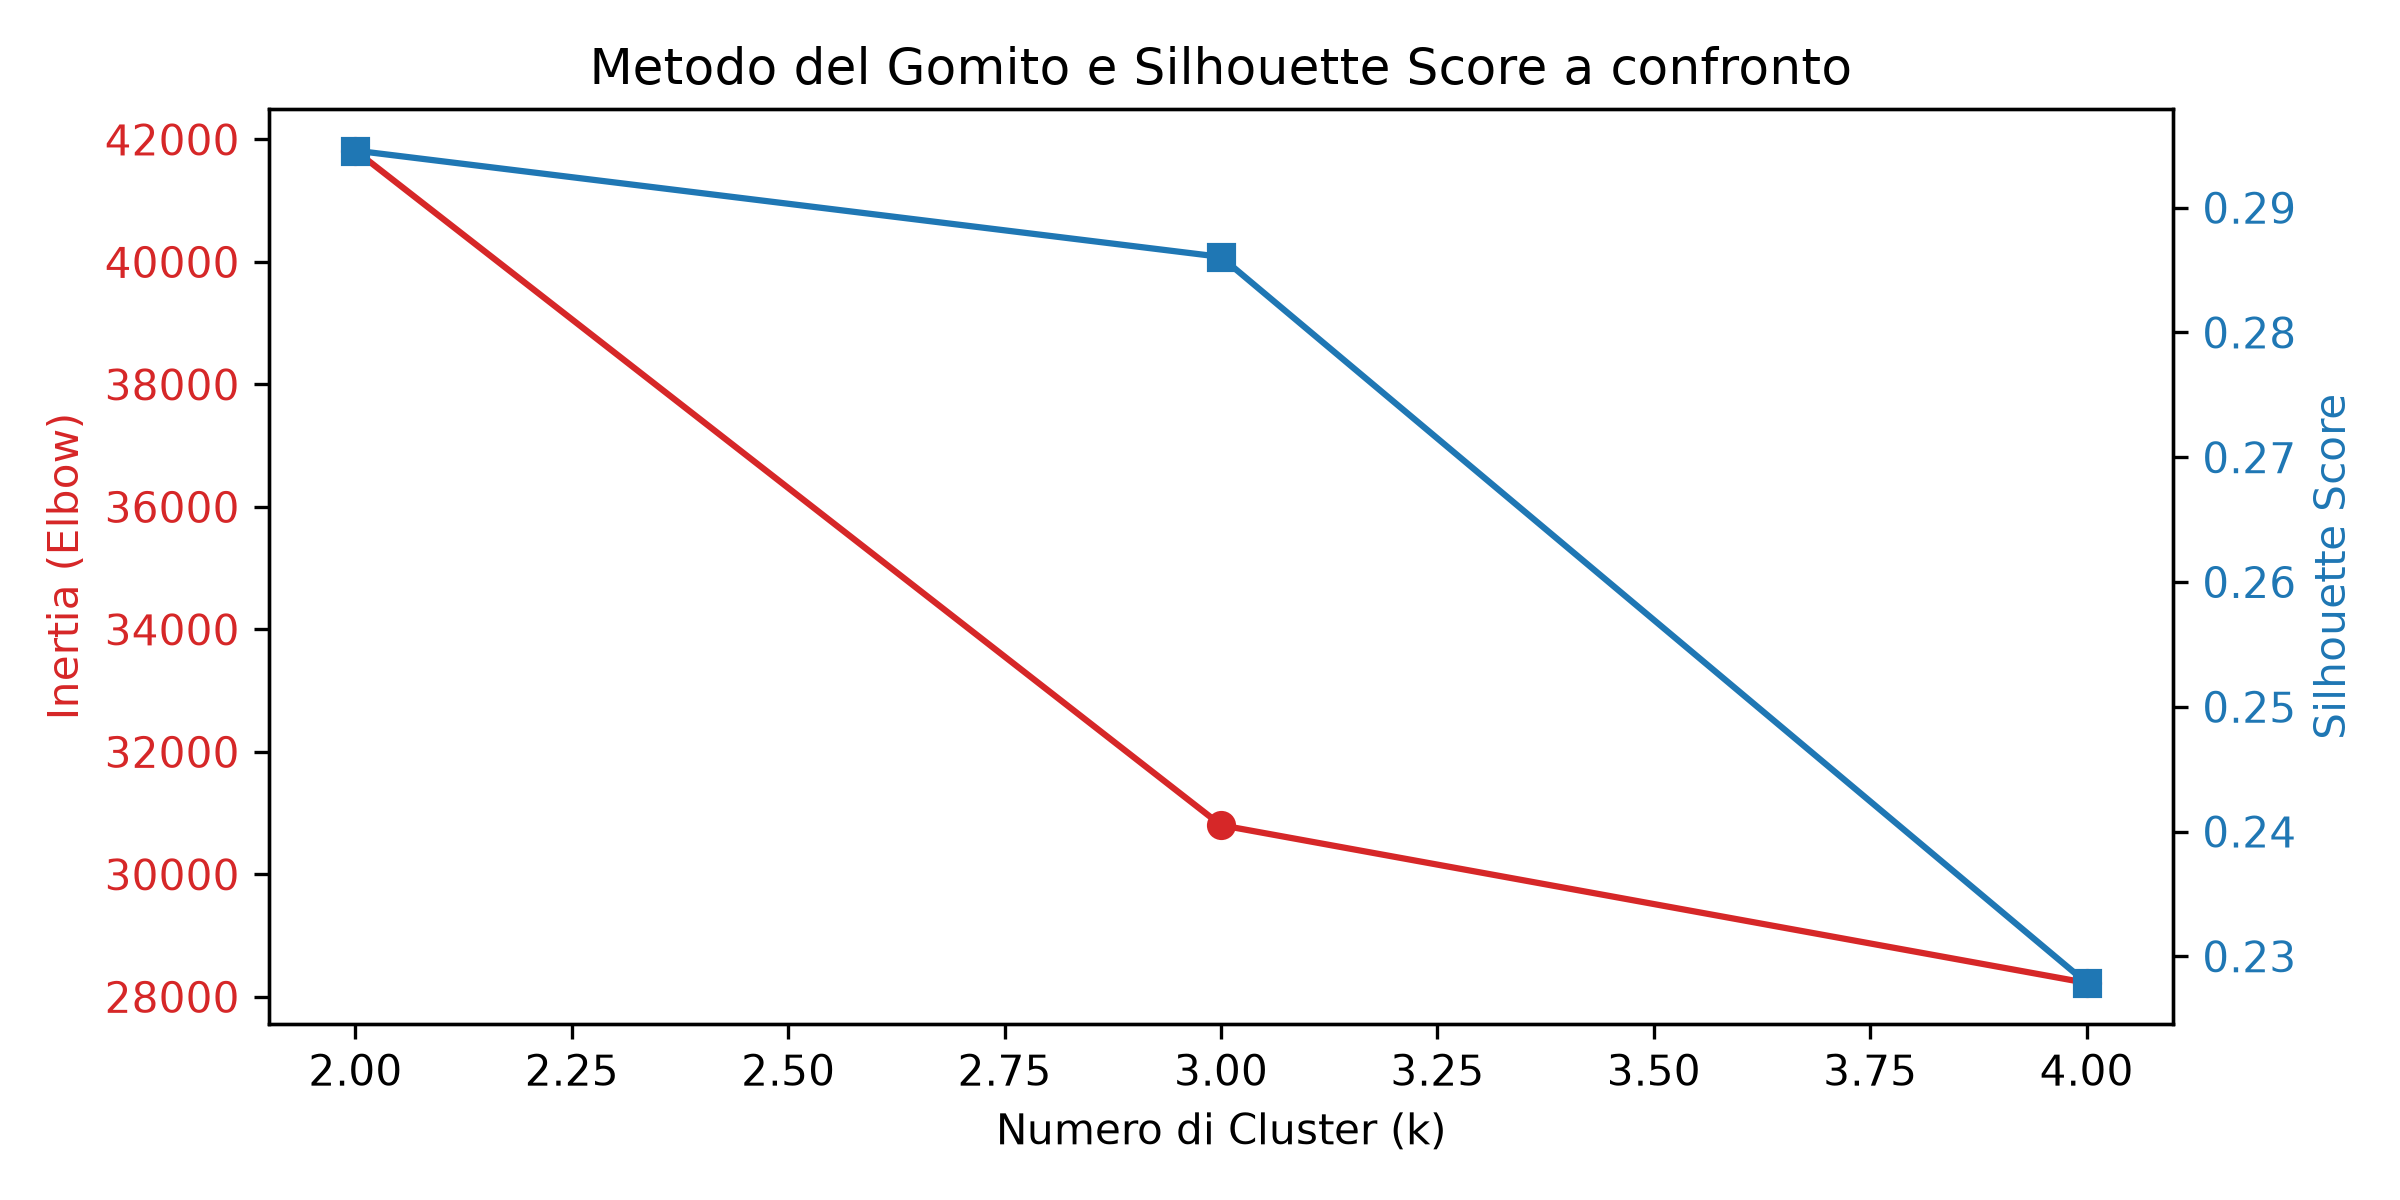
\includegraphics[width=\textwidth]{../grafici/clustering_evaluation.png}
      \begin{center}\scriptsize \textbf{Grafico}: Silhouette e Inertia indicano che $k=2$ è ottimale.\end{center}
    \end{column}
  \end{columns}
\end{frame}

% Slide 5: I Modelli di Classificazione Scelti
\begin{frame}{4. I Modelli di Predizione e gli Scenari}
  \small
  Abbiamo addestrato 3 modelli con filosofie diverse per capire se un cliente abbandonerà:
  \vspace{0.2cm}
  \begin{columns}
    \begin{column}{0.31\textwidth}
      \begin{block}{1. Regressione Logistica}
        \scriptsize
        \textbf{Baseline semplice.} Mappa i calcoli lineari in una probabilità [0, 1] tramite la funzione \textbf{Sigmoide}.
      \end{block}
    \end{column}
    \begin{column}{0.31\textwidth}
      \begin{block}{2. Decision Tree}
        \scriptsize
        \textbf{Modello a regole (IF-THEN).} Sceglie gli split migliori tramite l'indice di Gini. \texttt{max\_depth=5} per regolarizzare.
      \end{block}
    \end{column}
    \begin{column}{0.31\textwidth}
      \begin{block}{3. MLP (Rete Neurale)}
        \scriptsize
        \textbf{Rete non lineare complessa.} Usa strati nascosti con attivazione \textbf{ReLU} e \textbf{Sigmoide} in uscita per decidere.
      \end{block}
    \end{column}
  \end{columns}
  \vspace{0.4cm}
  Confrontati in due scenari:
  \begin{itemize}
    \item \textbf{Scenario A (Senza Cluster)}: solo variabili di partenza.
    \item \textbf{Scenario B (Con Cluster)}: aggiunta del cluster di k-Means come feature extra, per vedere se aiuta a predire il churn.
  \end{itemize}
\end{frame}

% Slide 6: Risultati Sperimentali
\begin{frame}{5. Tabella dei Risultati}
  Confronto tra lo Scenario \textbf{Senza Cluster} e lo Scenario \textbf{Con Cluster} (aggiunto come feature).
  \vspace{0.2cm}
  \begin{table}
    \centering
    \caption{Accuratezza, Recall (Richiamo dei clienti a rischio) e AUC su Train e Test.}
    \resizebox{0.9\textwidth}{!}{
      \begin{tabular}{llcccccc}
        \toprule
         & & \multicolumn{2}{c}{\textbf{Accuracy}} & \multicolumn{2}{c}{\textbf{Recall}} & \multicolumn{2}{c}{\textbf{AUC}} \\
        \cmidrule(lr){3-4} \cmidrule(lr){5-6} \cmidrule(lr){7-8}
        \textbf{Modello} & \textbf{Feature Scenario} & \textbf{Train} & \textbf{Test} & \textbf{Train} & \textbf{Test} & \textbf{Train} & \textbf{Test} \\
        \midrule
        Logistic Regression & Senza Cluster & 0.8053 & 0.8062 & 0.5485 & 0.5588 & 0.8492 & 0.8422 \\
        Logistic Regression & Con Cluster & 0.8051 & 0.8055 & 0.5485 & 0.5588 & 0.8492 & 0.8423 \\
        \midrule
        Decision Tree & Senza Cluster & 0.8023 & 0.7942 & 0.5612 & 0.5401 & 0.8476 & 0.8267 \\
        Decision Tree & Con Cluster & 0.8023 & 0.7942 & 0.5612 & 0.5401 & 0.8476 & 0.8267 \\
        \midrule
        Multi-Layer Perceptron (MLP) & Senza Cluster & 0.9143 & 0.7495 & 0.7813 & 0.4278 & 0.9656 & 0.7844 \\
        \rowcolor{unimeblue!10}
        Multi-Layer Perceptron (MLP) & Con Cluster & 0.9104 & 0.7360 & 0.9097 & \textbf{0.5829} & 0.9722 & 0.7846 \\
        \bottomrule
      \end{tabular}
    }
  \end{table}
  \vspace{0.1cm}
  \begin{itemize}
    \item \textbf{Cosa notare:} L'MLP con l'aggiunta del cluster fa salire la Recall di Test del \textbf{+15.5\%} (da 0.4278 a 0.5829).
  \end{itemize}
\end{frame}

% Slide 7: Albero di Decisione (Visualizzazione)
\begin{frame}{6. Regole dell'Albero di Decisione}
  \begin{columns}
    \begin{column}{0.48\textwidth}
      L'Albero di Decisione è trasparente (\textbf{white-box}):
      \vspace{0.2cm}
      \begin{itemize}
        \item \textbf{Scatole nell'albero}: contengono la regola di split, l'impurezza (\textbf{gini}), i clienti rimasti (\textbf{samples}) e il conteggio delle classi (\textbf{value}).
        \item \textbf{Colori}: i nodi sono \textbf{blu} se prevale chi rimane (classe 0) e \textbf{arancione} se prevale chi se ne va (classe 1). Più il colore è scuro e intenso, più il nodo è puro.
        \item \textbf{Regola chiave}: lo split iniziale avviene su \textbf{Contract\_Month-to-month}. Chi ha un contratto mensile ed è iscritto da poco (tenure bassa) ha un rischio di abbandono altissimo.
      \end{itemize}
    \end{column}
    \begin{column}{0.5\textwidth}
      \centering
      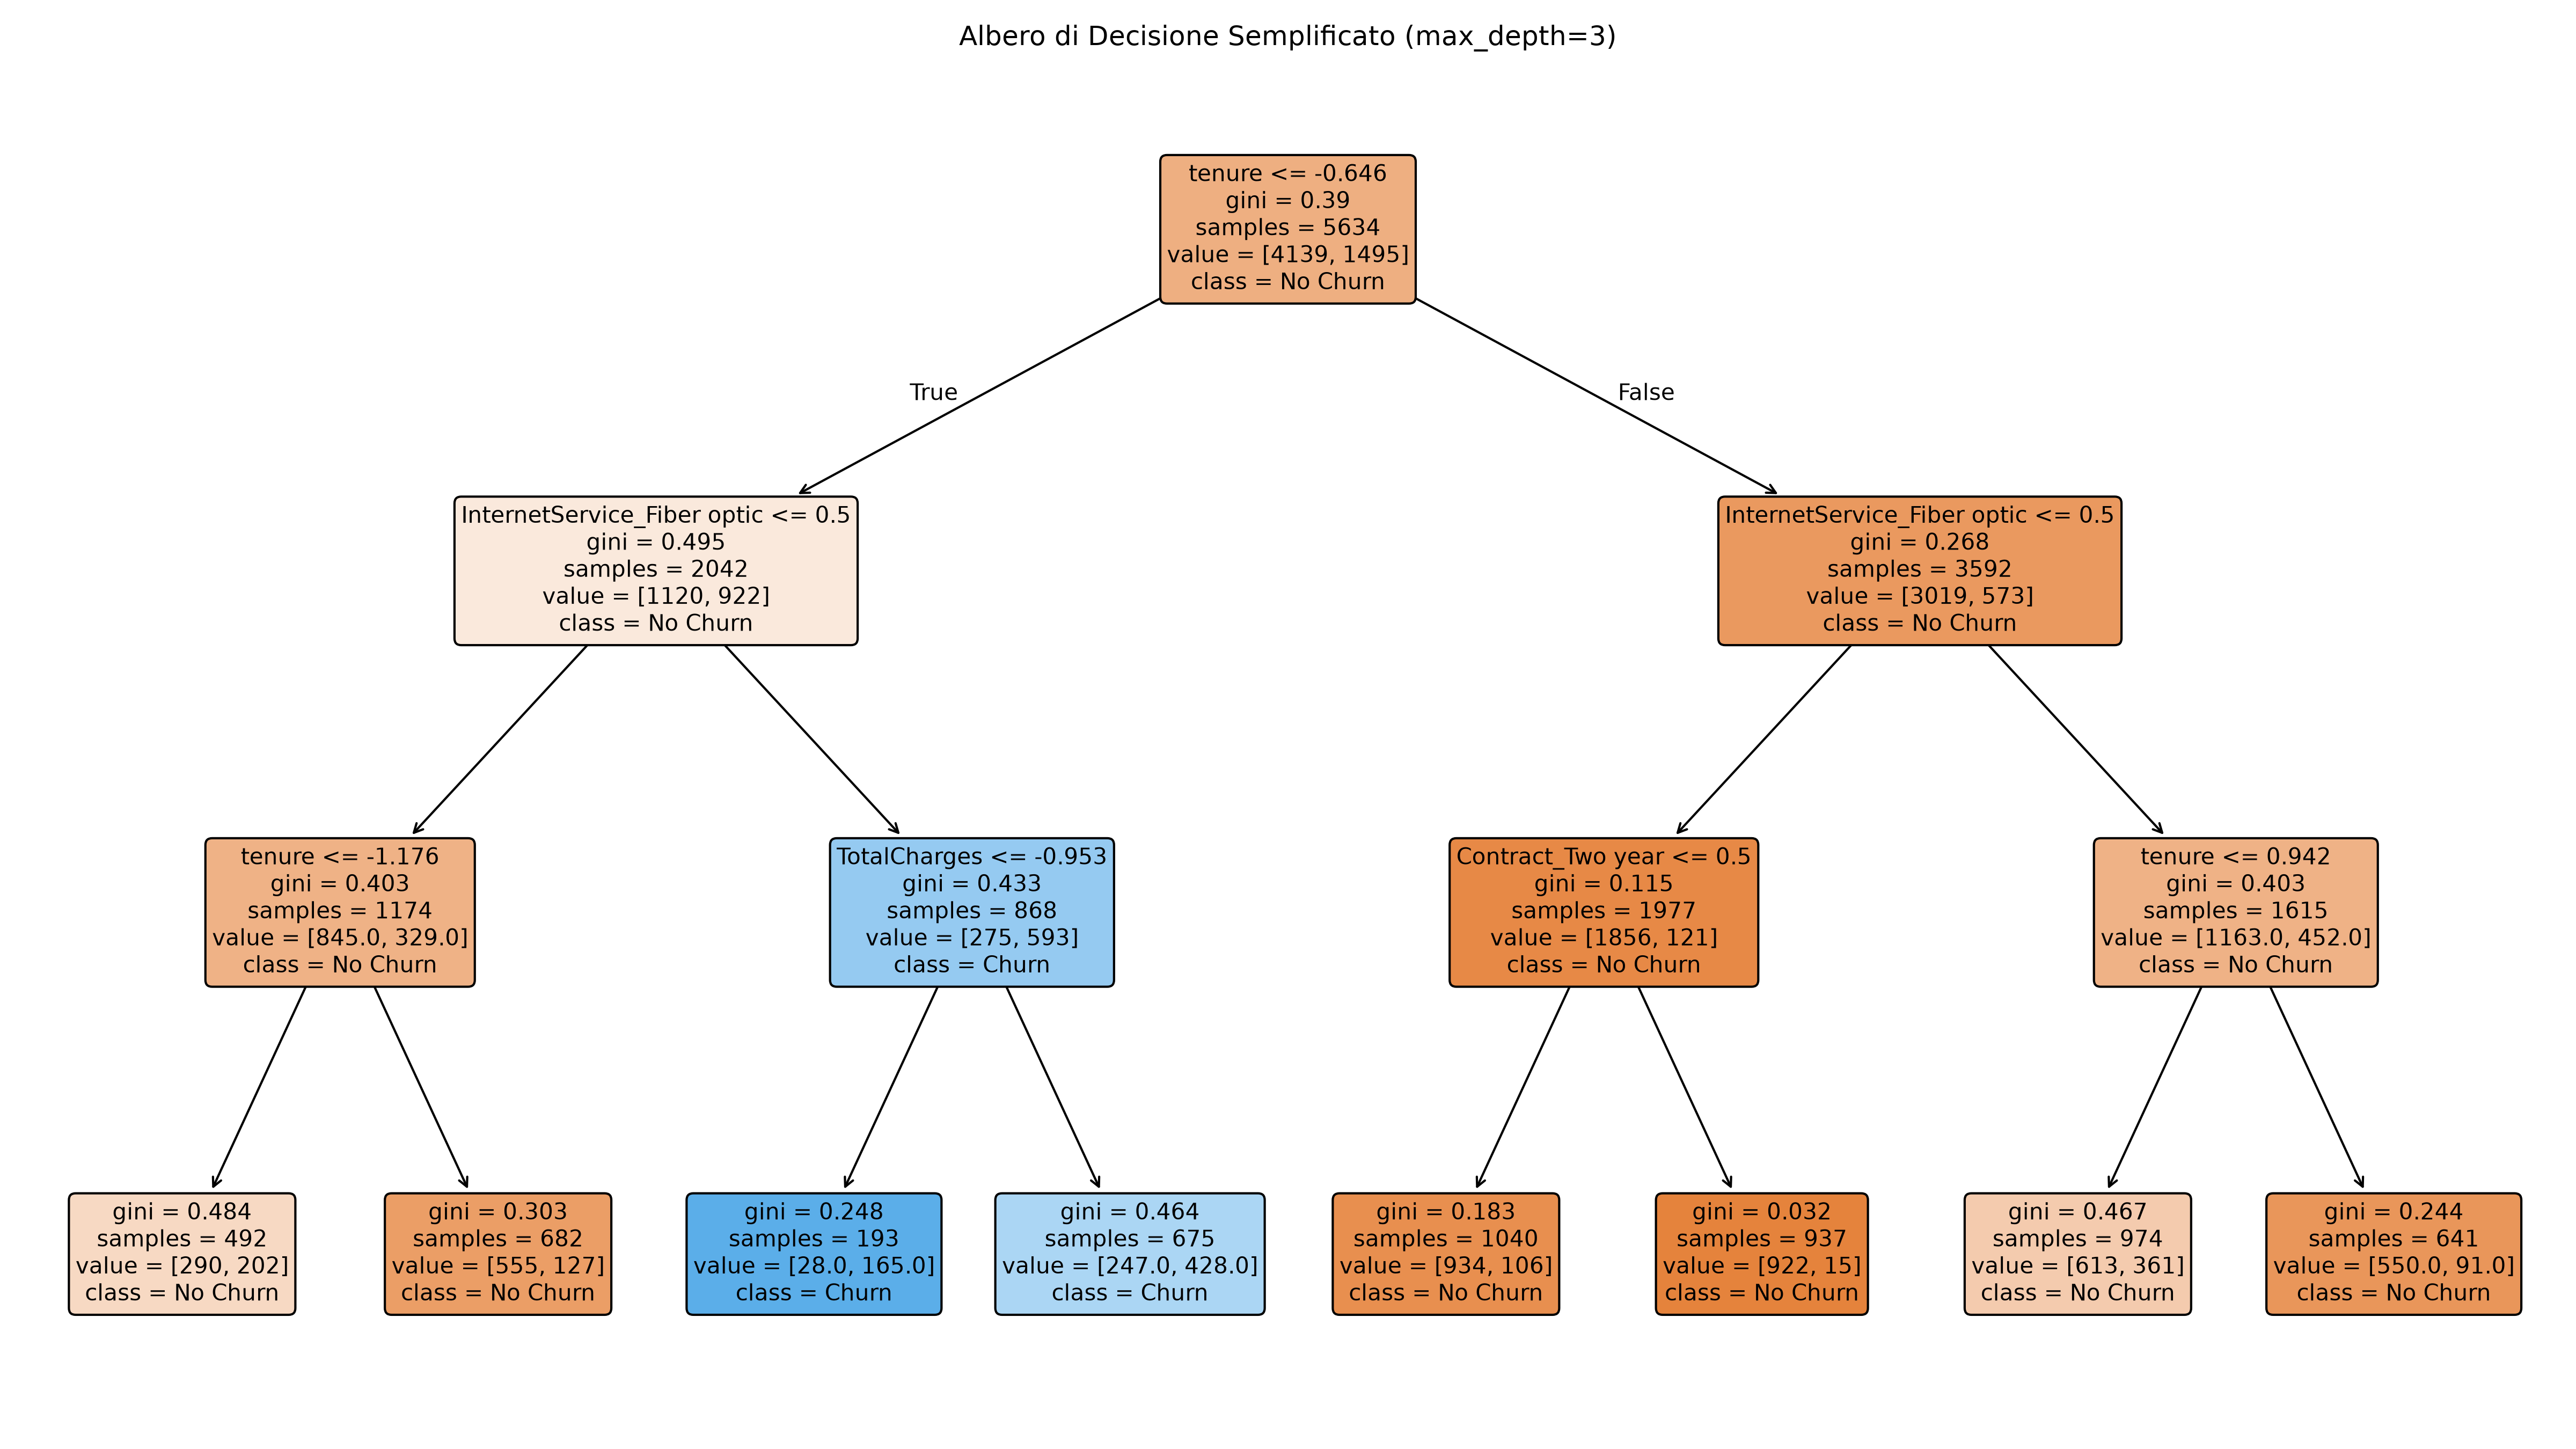
\includegraphics[width=\textwidth]{../grafici/decision_tree_vis.png}
      \begin{center}\scriptsize \textbf{Grafico}: Struttura a quiz dell'albero semplificato.\end{center}
    \end{column}
  \end{columns}
\end{frame}

% Slide 8: Overfitting dell'MLP e Importanza Feature
\begin{frame}{7. Overfitting, Underfitting e Importanza Feature}
  \begin{columns}
    \begin{column}{0.52\textwidth}
      \textbf{Overfitting vs Underfitting:}
      \begin{itemize}
        \item Non c'è underfitting: i modelli catturano bene il segnale ($\approx$ 80\% accuratezza).
        \item L'MLP soffre di \textbf{forte overfitting}: impara a memoria i dati di Train (91\%) ma crolla sul Test (73.6%).
      \end{itemize}
      \vspace{0.2cm}
      \textbf{L'utilità del Cluster:}
      \begin{itemize}
        \item Il cluster calcolato con k-Means figura nella top 10 delle feature importanti dell'albero di decisione.
        \item Funge da guida per i neuroni dell'MLP: nello Scenario B la Recall sale dal 42.8\% al \textbf{58.3\%} (\textbf{+15.5\%}).
      \end{itemize}
    \end{column}
    \begin{column}{0.45\textwidth}
      \centering
      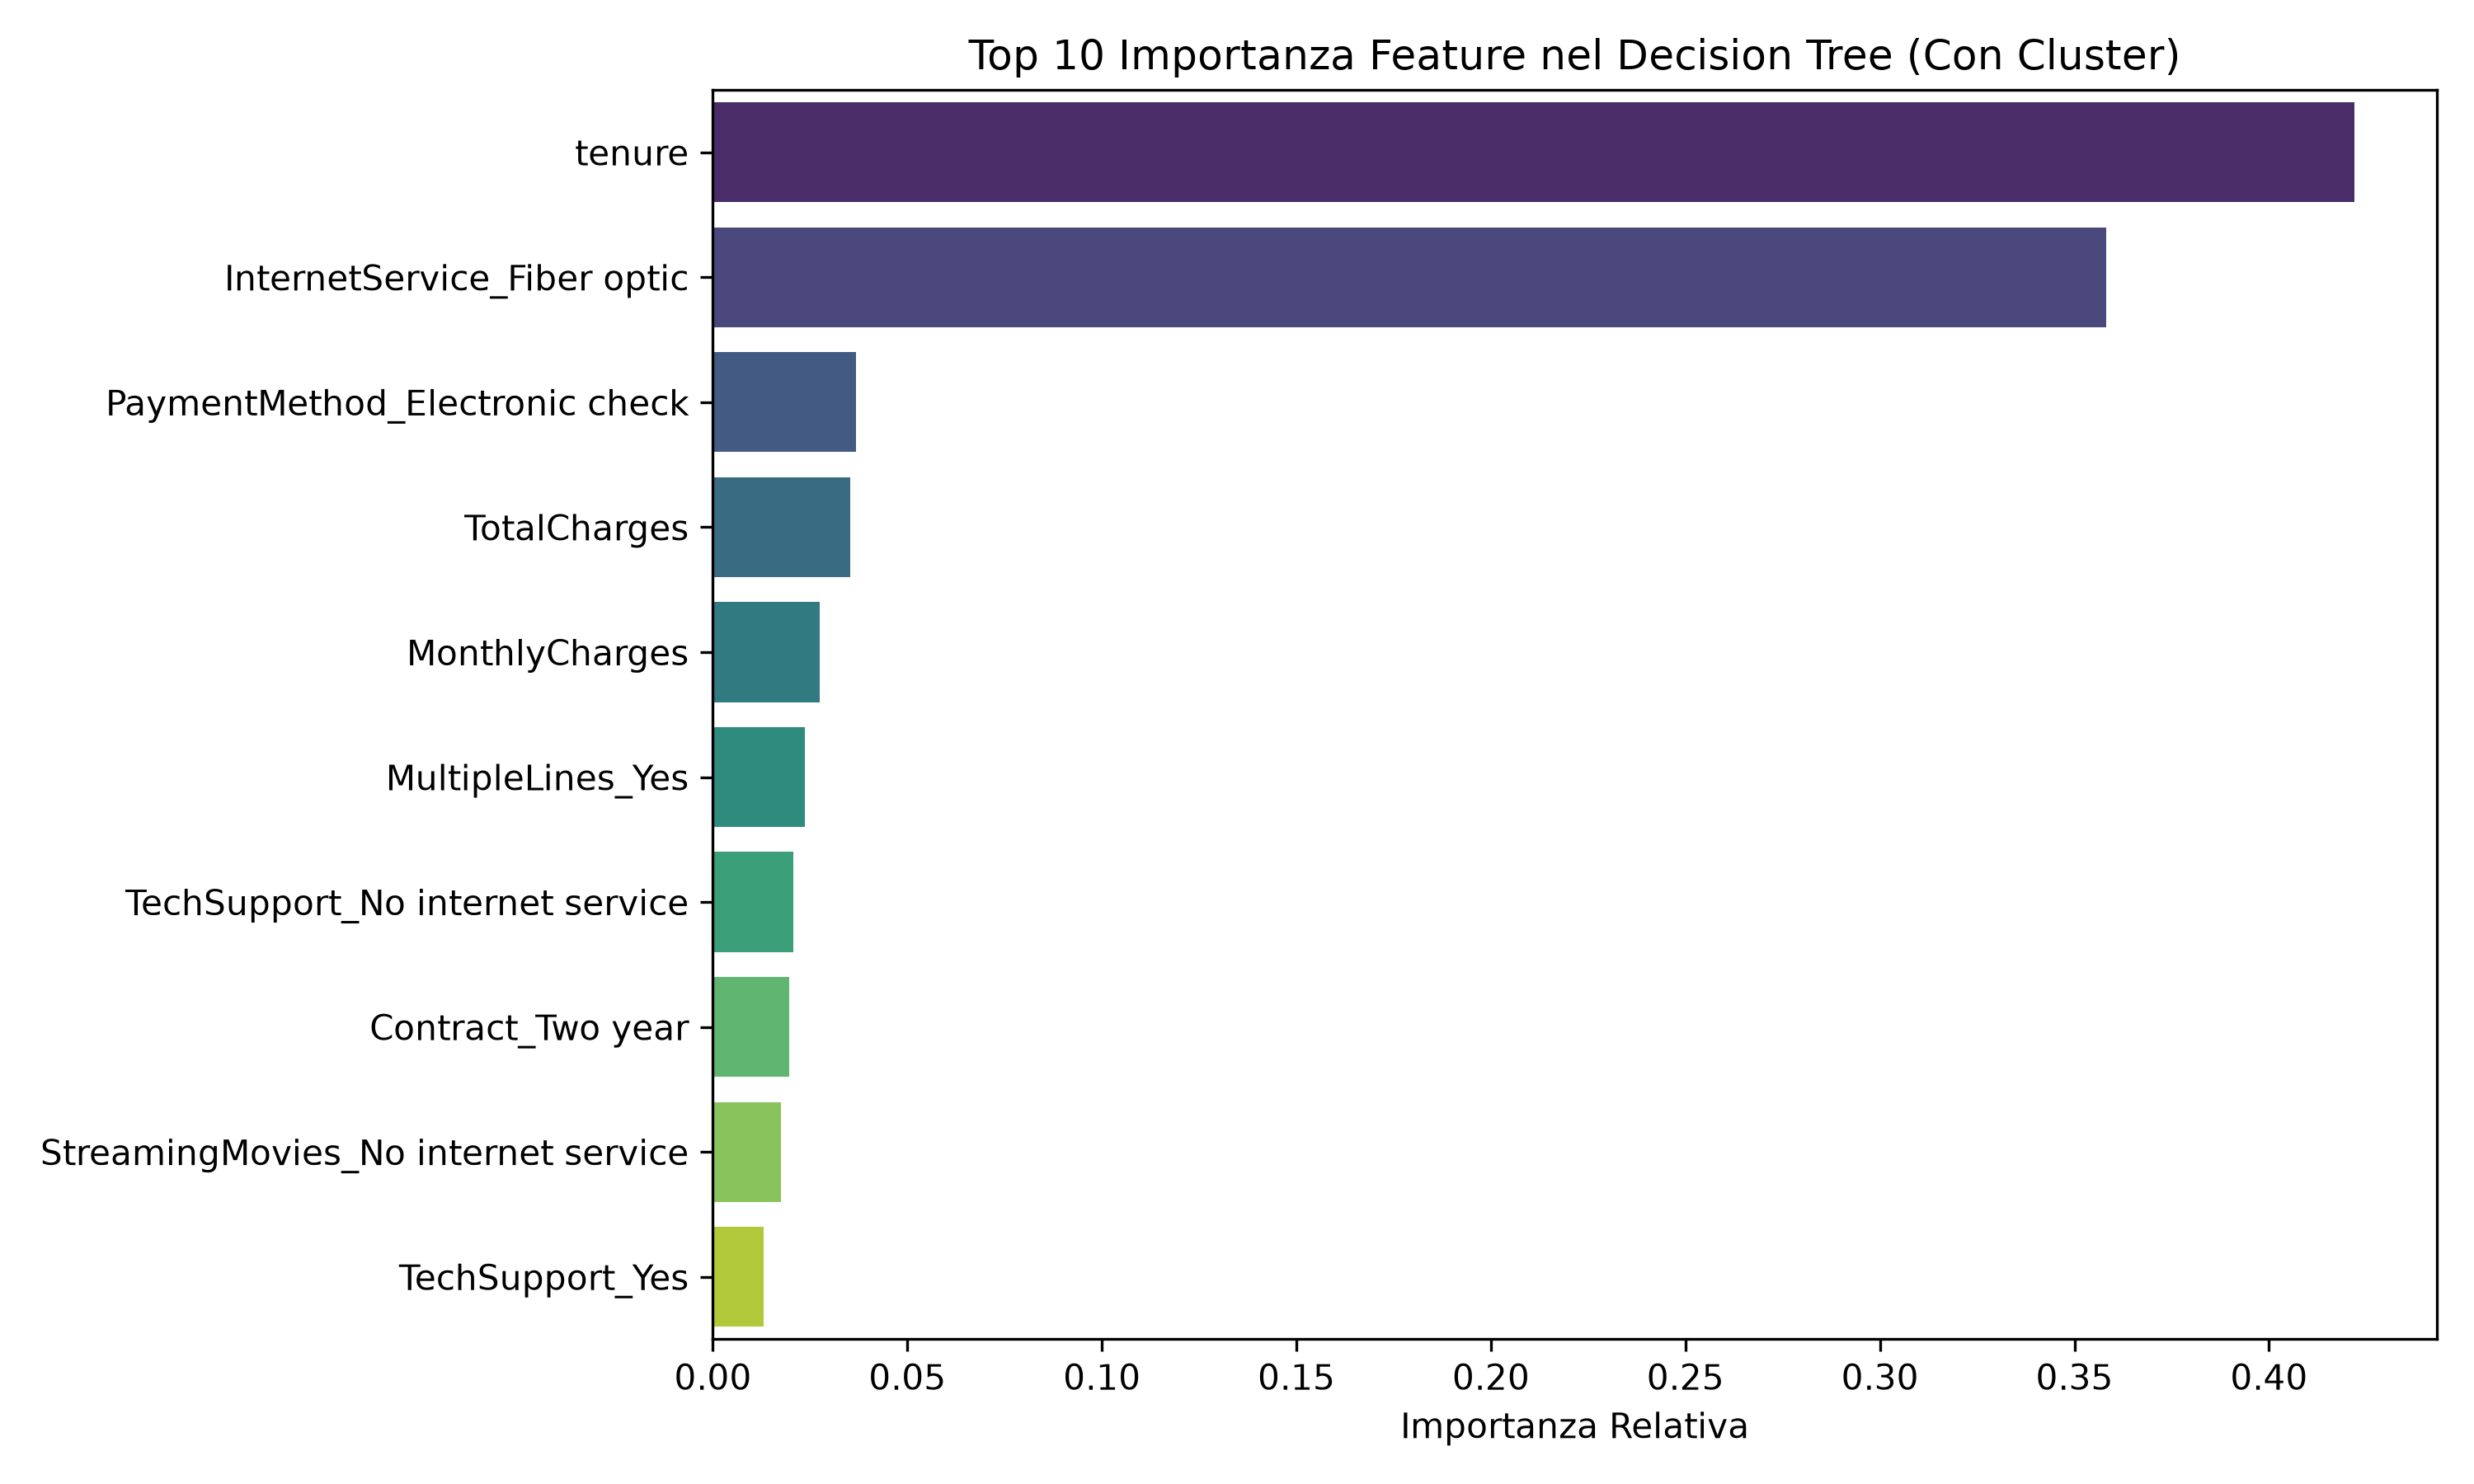
\includegraphics[width=\textwidth]{../grafici/feature_importances.png}
      \begin{center}\scriptsize \textbf{Grafico}: Le caratteristiche più importanti (contratto mensile, tenure, fibra, e il nostro Cluster).\end{center}
    \end{column}
  \end{columns}
\end{frame}

% Slide 9: Conclusioni
\begin{frame}{8. Cosa impariamo da questo Progetto?}
  \textbf{Conclusioni Chiave:}
  \begin{itemize}
    \item Il \textbf{Clustering} (non supervisionato) ha diviso i clienti in due profili commerciali chiari (spesa bassa e fedeli vs. spesa alta e volatili).
    \item Inserire questo profilo come feature ha aiutato la \textbf{Rete Neurale (MLP)} a identificare molti più clienti a rischio di abbandono sul Test Set (Recall +15.5\%).
  \end{itemize}
  \vspace{0.3cm}
  \textbf{Sviluppi Futuri per migliorare:}
  \begin{itemize}
    \item Utilizzare tecniche per bilanciare i dati (SMOTE) ed evitare l'overfitting dell'MLP.
    \item Provare modelli ensemble come il \textbf{Random Forest}.
  \end{itemize}
  \vspace{0.4cm}
  \centering
  \textbf{\large Grazie per l'attenzione!}
\end{frame}

\end{document}
